\documentclass[aspectratio=169]{beamer}

\usepackage{fontspec}
\usepackage{microtype}
\usepackage{fontawesome}
\usepackage{tikz}
\usetikzlibrary{positioning, calc, patterns}
\usetikzlibrary{overlay-beamer-styles}
\setbeamertemplate{frametitle}[default][center]

\hypersetup{
    colorlinks,
    linkcolor=red,
    pdftitle={Patterns of interview solutions},
    pdfpagemode=FullScreen,
    }

\setmonofont{JetBrainsMono}[
    Path=./static/fonts/jetbrains/,
    Scale=0.85,
    Extension = .ttf,
    UprightFont=*-Regular,
    BoldFont=*-Bold,
    ItalicFont=*-Italic,
    BoldItalicFont=*-BoldItalic
    ]
    
\setsansfont{Asap}[
    Path=./static/fonts/asap/,
    Scale=0.9,
    Extension = .ttf,
    UprightFont=*-Regular,
    BoldFont=*-Bold,
    ItalicFont=*-Italic,
    BoldItalicFont=*-BoldItalic
    ]

\usepackage[newfloat=true]{minted}
\usemintedstyle{xcode}
\beamertemplatenavigationsymbolsempty

\setbeamertemplate{footline}{\begin{center}\quad\insertframenumber\strut\quad\end{center}}
\setbeamerfont{footline}{size=\large}

\title{Patterns of interview solutions}
\author{Šimon Tóth}

\begin{document}

\frame{\titlepage}

%\if{0}

\begin{frame}{}
  \begin{columns}
      \begin{column}{0.35\textwidth}
          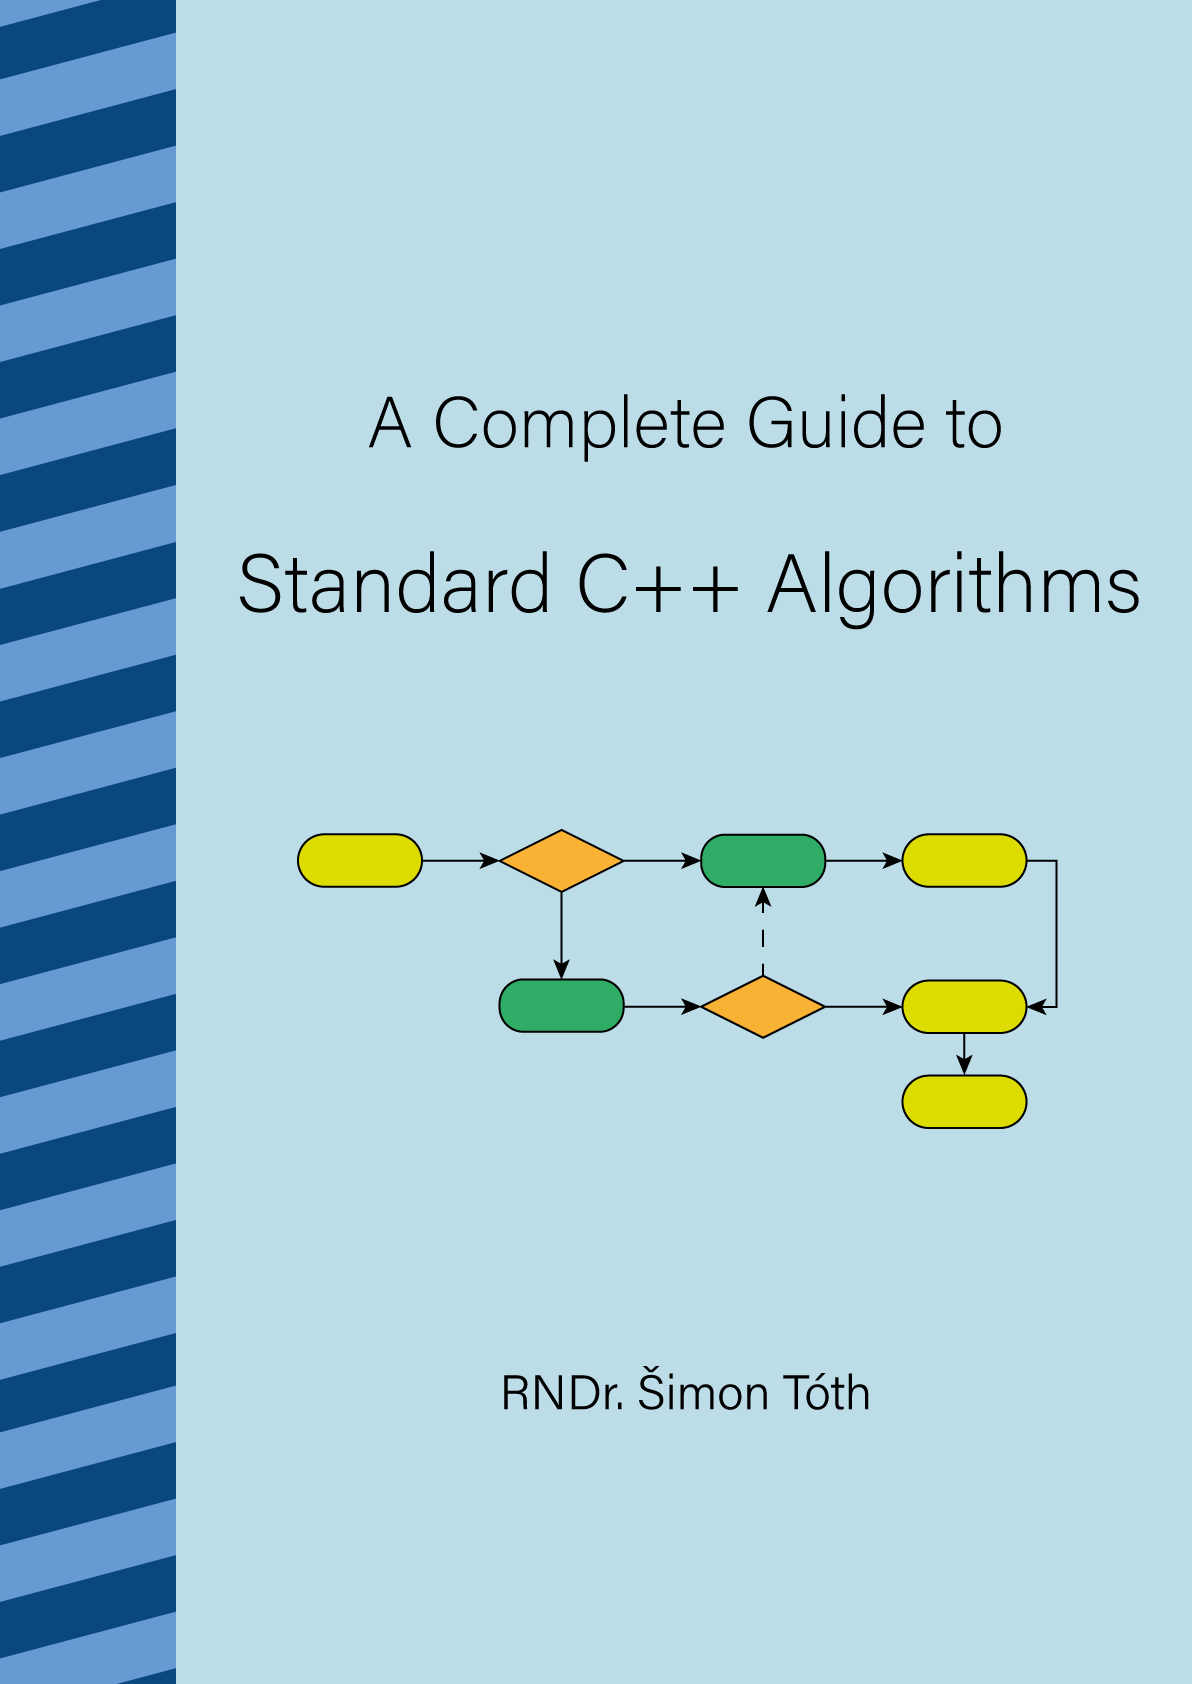
\includegraphics[height=0.8\textheight]{static/book_cover_algo.png}
      \end{column}
      \begin{column}{0.6\textwidth}
          \begin{itemize}
              \item Free on GitHub:\\
                  \href{https://github.com/HappyCerberus/book-cpp-algorithms}{HappyCerberus/book-cpp-algorithms}
              \item Donate to EFF on LeanPub:\\
                  \href{https://leanpub.com/cpp-algorithms-guide}{leanpub.com/cpp-algorithms-guide}
          \end{itemize}
      \end{column}
  \end{columns}
\end{frame}

\begin{frame}{}
  \begin{columns}
      \begin{column}{0.35\textwidth}
          
\includegraphics[height=0.8\textheight]{static/book_cover_interview.png}
      \end{column}
      \begin{column}{0.6\textwidth}
          \begin{itemize}
              \item Source on GitHub:\\
                  \href{https://github.com/HappyCerberus/cpp-coding-interview}{HappyCerberus/cpp-coding-interview}
              \item Community version free,\\or donate to EFF on LeanPub:\\
                  \href{https://leanpub.com/cpp-coding-interview}{leanpub.com/cpp-coding-interview}
          \end{itemize}
      \end{column}
  \end{columns}
\end{frame}

\begin{frame}{Daily bit(e) of C++}
  \begin{itemize}
    \item \href{https://www.linkedin.com/in/simontoth}{linkedin.com/in/simontoth}
    \item \href{https://hachyderm.io/@simontoth}{hachyderm.io/@simontoth}
    \item \href{https://simontoth.substack.com/}{simontoth.substack.com}
    \item \href{https://medium.com/@simontoth}{medium.com/@simontoth}
  \end{itemize}
  \vspace{1em}
  \pause Starting 1st December, the series will switch to Advent of Code 2023 solutions.
\end{frame}

\begin{frame}[c]
\begin{center}
  \huge What is the point of this problem?
\end{center}
\end{frame}

\begin{frame}[c]
\begin{center}
  \huge What is the point of the solution?
\end{center}
\end{frame}

\begin{frame}[c]
  \begin{center}
    \huge Making good use of the standard library
  \end{center}
\end{frame}

\begin{frame}{Algorithms}
  \pause
  \tiny
  \begin{columns}
    \begin{column}{.33\textwidth}
      \begin{itemize}
        \item{\mintinline{cpp}{all_of}}
        \item{\mintinline{cpp}{any_of}}
        \item{\mintinline{cpp}{none_of}}
        \item{\mintinline{cpp}{for_each}}
        \item{\mintinline{cpp}{for_each_n}}
        \item{\mintinline{cpp}{count}}
        \item{\mintinline{cpp}{count_if}}
        \item{\mintinline{cpp}{mismatch}}
        \item{\mintinline{cpp}{find}}
        \item{\mintinline{cpp}{find_if}}
        \item{\mintinline{cpp}{find_if_not}}
        \item{\mintinline{cpp}{ranges::find_last}}
        \item{\mintinline{cpp}{ranges::find_last_if}}
        \item{\mintinline{cpp}{ranges::find_last_if_not}}
        \item{\mintinline{cpp}{find_end}}
        \item{\mintinline{cpp}{find_first_of}}
        \item{\mintinline{cpp}{adjacent_find}}
        \item{\mintinline{cpp}{search}}
        \item{\mintinline{cpp}{search_n}}
      \end{itemize}
    \end{column}
    \begin{column}{.33\textwidth}
      \begin{itemize}
        \item{\mintinline{cpp}{ranges::starts_with}}
        \item{\mintinline{cpp}{ranges::ends_with}}
        \item{\mintinline{cpp}{copy}}
        \item{\mintinline{cpp}{copy_if}}
        \item{\mintinline{cpp}{copy_n}}
        \item{\mintinline{cpp}{copy_backward}}
        \item{\mintinline{cpp}{move}}
        \item{\mintinline{cpp}{move_backward}}
        \item{\mintinline{cpp}{fill}}
        \item{\mintinline{cpp}{fill_n}}
        \item{\mintinline{cpp}{transform}}
        \item{\mintinline{cpp}{generate}}
        \item{\mintinline{cpp}{generate_n}}
        \item{\mintinline{cpp}{remove}}
        \item{\mintinline{cpp}{remove_if}}
        \item{\mintinline{cpp}{remove_copy}}
        \item{\mintinline{cpp}{remove_copy_if}}
        \item{\mintinline{cpp}{replace}}
        \item{\mintinline{cpp}{replace_if}}
      \end{itemize}
    \end{column}
    \begin{column}{.33\textwidth}
      \begin{itemize}
        \item{\mintinline{cpp}{replace_copy}}
        \item{\mintinline{cpp}{replace_copy_if}}
        \item{\mintinline{cpp}{swap}}
        \item{\mintinline{cpp}{swap_ranges}}
        \item{\mintinline{cpp}{iter_swap}}
        \item{\mintinline{cpp}{reverse}}
        \item{\mintinline{cpp}{reverse_copy}}
        \item{\mintinline{cpp}{rotate}}
        \item{\mintinline{cpp}{rotate_copy}}
        \item{\mintinline{cpp}{shift_left}}
        \item{\mintinline{cpp}{shift_right}}
        \item{\mintinline{cpp}{shuffle}}
        \item{\mintinline{cpp}{sample}}
        \item{\mintinline{cpp}{unique}}
        \item{\mintinline{cpp}{unique_copy}}
        \item{\mintinline{cpp}{is_partitioned}}
        \item{\mintinline{cpp}{partition}}
        \item{\mintinline{cpp}{partition_copy}}
        \item{\mintinline{cpp}{stable_partition}}
      \end{itemize}
    \end{column}
  \end{columns}
\end{frame}

\begin{frame}{Algorithms}
  \tiny
  \begin{columns}
    \begin{column}{.33\textwidth}
      \begin{itemize}
        \item{\mintinline{cpp}{partition_point}}
        \item{\mintinline{cpp}{is_sorted}}
        \item{\mintinline{cpp}{is_sorted_until}}
        \item{\mintinline{cpp}{sort}}
        \item{\mintinline{cpp}{partial_sort}}
        \item{\mintinline{cpp}{partial_sort_copy}}
        \item{\mintinline{cpp}{stable_sort}}
        \item{\mintinline{cpp}{nth_element}}
        \item{\mintinline{cpp}{lower_bound}}
        \item{\mintinline{cpp}{upper_bound}}
        \item{\mintinline{cpp}{binary_search}}
        \item{\mintinline{cpp}{equal_range}}
        \item{\mintinline{cpp}{merge}}
        \item{\mintinline{cpp}{inplace_merge}}
        \item{\mintinline{cpp}{includes}}
        \item{\mintinline{cpp}{set_difference}}
        \item{\mintinline{cpp}{set_intersection}}
        \item{\mintinline{cpp}{set_symmetric_difference}}
        \item{\mintinline{cpp}{set_union}}
      \end{itemize}
    \end{column}
    \begin{column}{.33\textwidth}
      \begin{itemize}
        \item{\mintinline{cpp}{is_heap}}
        \item{\mintinline{cpp}{is_heap_until}}
        \item{\mintinline{cpp}{make_heap}}
        \item{\mintinline{cpp}{push_heap}}
        \item{\mintinline{cpp}{pop_heap}}
        \item{\mintinline{cpp}{sort_heap}}
        \item{\mintinline{cpp}{max}}
        \item{\mintinline{cpp}{max_element}}
        \item{\mintinline{cpp}{min}}
        \item{\mintinline{cpp}{min_element}}
        \item{\mintinline{cpp}{minmax}}
        \item{\mintinline{cpp}{minmax_element}}
        \item{\mintinline{cpp}{clamp}}
        \item{\mintinline{cpp}{equal}}
        \item{\mintinline{cpp}{lexicographical_compare}}
        \item{\mintinline{cpp}{lexicographical_compare_three_way}}
        \item{\mintinline{cpp}{is_permutation}}
        \item{\mintinline{cpp}{next_permutation}}
        \item{\mintinline{cpp}{prev_permutation}}
      \end{itemize}
    \end{column}
    \begin{column}{.33\textwidth}
      \begin{itemize}
        \item{\mintinline{cpp}{iota}}
        \item{\mintinline{cpp}{accumulate}}
        \item{\mintinline{cpp}{inner_product}}
        \item{\mintinline{cpp}{adjacent_difference}}
        \item{\mintinline{cpp}{partial_sum}}
        \item{\mintinline{cpp}{reduce}}
        \item{\mintinline{cpp}{exclusive_scan}}
        \item{\mintinline{cpp}{inclusive_scan}}
        \item{\mintinline{cpp}{transform_reduce}}
        \item{\mintinline{cpp}{transform_exclusive_scan}}
        \item{\mintinline{cpp}{transform_inclusive_scan}}
        \item{\mintinline{cpp}{ranges::fold_left}}
        \item{\mintinline{cpp}{ranges::fold_left_first}}
        \item{\mintinline{cpp}{ranges::fold_right}}
        \item{\mintinline{cpp}{ranges::fold_right_last}}
        \item{\mintinline{cpp}{ranges::fold_left_with_iter}}
        \item{\mintinline{cpp}{ranges::fold_left_first_with_iter}}
        \item{\mintinline{cpp}{uninitialized_copy}}
        \item{\mintinline{cpp}{uninitialized_copy_n}}
      \end{itemize}
    \end{column}
  \end{columns}
\end{frame}

\begin{frame}{Algorithms}
  \tiny
  \begin{columns}
    \begin{column}{.33\textwidth}
      \begin{itemize}
        \item{\mintinline{cpp}{uninitialized_fill}}
        \item{\mintinline{cpp}{uninitialized_fill_n}}
        \item{\mintinline{cpp}{uninitialized_move}}
        \item{\mintinline{cpp}{uninitialized_move_n}}
        \item{\mintinline{cpp}{uninitialized_default_construct}}
        \item{\mintinline{cpp}{uninitialized_default_construct_n}}
        \item{\mintinline{cpp}{uninitialized_value_construct}}
        \item{\mintinline{cpp}{uninitialized_value_construct_n}}
        \item{\mintinline{cpp}{destroy}}
        \item{\mintinline{cpp}{destroy_n}}
        \item{\mintinline{cpp}{destroy_at}}
        \item{\mintinline{cpp}{construct_at}}
      \end{itemize}
    \end{column}
    \begin{column}{.33\textwidth}
    \end{column}
    \begin{column}{.33\textwidth}
    \end{column}
  \end{columns}
\end{frame}

\begin{frame}{Iterators and ranges}
  \begin{tikzpicture}[
    basenode/.style={rectangle, draw=red!60, fill=red!5, thick, minimum size=1cm, text depth=.0\baselineskip, text height=.7\baselineskip},
    centernode/.style={rectangle, draw=red!60, fill=red!5, thick, minimum size=1cm, text depth=.0\baselineskip, text height=.7\baselineskip},
    greynode/.style={rectangle, draw=black!60, fill=black!5, thick, minimum size=1cm, text depth=.0\baselineskip, text height=.7\baselineskip},
    overlay, remember picture
  ]
    \node[basenode](center) at (current page.center){};
    \node[basenode](l1)[left=0cm of center]{};
    \node[basenode](l2)[left=0cm of l1]{};
    \node[basenode](r1)[right=0cm of center]{};
    \node[greynode](r2)[right=0cm of r1]{};
    \node(begin)[below=1cm of l2]{begin};
    \node(end)[below=1cm of r2]{end};
    \draw[thick, ->](begin)--(l2);
    \draw[thick, ->](end)--(r2);
  \end{tikzpicture}
\end{frame}

\begin{frame}[fragile]{Iterators and ranges}
  \begin{minted}[escapeinside=||]{cpp}
    int data[] = {1,2,3,4,5};

    int* begin = data;
    int* end = begin + 5;

    for (int* it = begin; it != end; ++it) {
    }
  \end{minted}
  % https://compiler-explorer.com/z/h6GbK8Pbj
\end{frame}

\begin{frame}{Iterators and ranges}
  \begin{itemize}
    \item contiguous blocks of memory\\
    \mintinline{cpp}{std::vector}, \mintinline{cpp}{std::array}
    \item chunks of contiguous memory\\
    \mintinline{cpp}{std::deque}
    \item linked-lists and trees\\
    \mintinline{cpp}{std::list}, \mintinline{cpp}{std::map}, \mintinline{cpp}{std::unordered_map}
    \item streams\\
    \mintinline{cpp}{std::ostream}, \mintinline{cpp}{std::istream}
  \end{itemize}
\end{frame}

\begin{frame}[c]
  \begin{center}
    \LARGE The 126 algorithms
  \end{center}
\end{frame}

\begin{frame}{For-each 2/126}
  \begin{itemize}
    \item{\mintinline{cpp}{for_each}}
    \item{\mintinline{cpp}{for_each_n}}
  \end{itemize}
\end{frame}

\begin{frame}[fragile]{}
\begin{minted}[escapeinside=||]{cpp}
  std::vector<int> data{1,2,3,4,5};

  std::for_each(data.begin(), data.end(),
      [](auto &e) { });

  std::for_each_n(data.begin(), 3,
      [](auto &e) { });
\end{minted}
% https://compiler-explorer.com/z/TGd7Yb75e
\end{frame}

\begin{frame}{Uninitialized memory algorithms 16/126}
\footnotesize
 \begin{columns}
  \begin{column}{0.6\textwidth}
  \begin{itemize}
    \item{\mintinline{cpp}{uninitialized_copy}}
    \item{\mintinline{cpp}{uninitialized_copy_n}}
    \item{\mintinline{cpp}{uninitialized_fill}}
    \item{\mintinline{cpp}{uninitialized_fill_n}}
    \item{\mintinline{cpp}{uninitialized_move}}
    \item{\mintinline{cpp}{uninitialized_move_n}}
    \item{\mintinline{cpp}{uninitialized_default_construct}}
    \item{\mintinline{cpp}{uninitialized_default_construct_n}}
    \item{\mintinline{cpp}{uninitialized_value_construct}}
    \item{\mintinline{cpp}{uninitialized_value_construct_n}}
    \item{\mintinline{cpp}{destroy}}
    \item{\mintinline{cpp}{destroy_n}}
  \end{itemize}
  \end{column}
  \begin{column}{0.4\textwidth}
  \begin{itemize}
    \item{\mintinline{cpp}{construct_at}}
    \item{\mintinline{cpp}{destroy_at}}
  \end{itemize}
  \end{column}
\end{columns}
\end{frame}

\begin{frame}{Heap algorithms 22/126}
  \begin{itemize}
    \item{\mintinline{cpp}{is_heap}}
    \item{\mintinline{cpp}{is_heap_until}}
    \item{\mintinline{cpp}{make_heap}}
    \item{\mintinline{cpp}{push_heap}}
    \item{\mintinline{cpp}{pop_heap}}
    \item{\mintinline{cpp}{sort_heap}}
  \end{itemize}
\end{frame}

\begin{frame}{Swaps 25/126}
  \begin{itemize}
    \item{\mintinline{cpp}{swap}}
    \item{\mintinline{cpp}{swap_ranges}}
    \item{\mintinline{cpp}{iter_swap}}
  \end{itemize}
\end{frame}

\begin{frame}[fragile]{}
\begin{minted}[escapeinside=||]{cpp}
void func(auto& a, auto& b) {
    using std::swap;
    swap(a,b);
}

|\pause|void func_ranges(auto& a, auto& b) {
    std::ranges::swap(a,b);
}
\end{minted}
% https://compiler-explorer.com/z/9hGd77e1o
\end{frame}

\begin{frame}{Sorting 27/126}
  \begin{itemize}
    \item{\mintinline{cpp}{sort}}
    \item{\mintinline{cpp}{stable_sort}}
  \end{itemize}
\end{frame}

\begin{frame}[fragile]{}
\begin{columns}
\begin{column}{0.4\textwidth}
\begin{minted}[escapeinside=||]{cpp}
struct Record {
    std::string name;
    uint64_t rank;
};

std::vector<Record> data{
    {"Banana", 2},
    {"Watermelon", 1},
    {"Apple", 1},
    {"Pear", 3}
};
\end{minted}
\end{column}
\pause
\vrule{}
\begin{column}{0.6\textwidth}
\begin{minted}[escapeinside=||]{cpp}
std::stable_sort(data.begin(), data.end(), 
    [](const auto& l, const auto& r) {
        return l.name < r.name;
    });
// Apple, Banana, Pear, Watermelon

std::stable_sort(data.begin(), data.end(), 
    [](const auto& l, const auto& r) {
        return l.rank < r.rank;
    });
// Apple, Watermelon, Banana, Pear
\end{minted}
\end{column}
\end{columns}
\end{frame}

\begin{frame}[fragile]{}
\begin{minted}[escapeinside=||]{cpp}
std::stable_sort(data.begin(), data.end(), 
    [](const auto& l, const auto& r) {
        return l.rank < r.rank;
    });

|\pause|std::ranges::stable_sort(data, 
    [](const auto& l, const auto& r) {
        return l.rank < r.rank;
    });

|\pause|std::ranges::stable_sort(data,
    std::less<>{}, &Record::rank);
\end{minted}
%https://compiler-explorer.com/z/7h9bc3fTb
\end{frame}

\begin{frame}{Sorting 29/126}
  \begin{itemize}
    \item{\mintinline{cpp}{partial_sort}}
    \item{\mintinline{cpp}{partial_sort_copy}}
  \end{itemize}
\end{frame}

\begin{frame}[fragile]{}
\begin{minted}[escapeinside=||]{cpp}
std::list<int> data{4,1,5,3,2};
std::vector<int> out(3);

std::ranges::partial_sort_copy(data, out);
// out == {1,2,3}

|\pause|const std::vector<int> immutable{4,1,5,3,2};
std::ranges::partial_sort_copy(immutable, out);
// out == {1,2,3}
\end{minted}
%https://compiler-explorer.com/z/d1c8rnfc3
\end{frame}

\begin{frame}{Sorting 31/126}
  \begin{itemize}
    \item{\mintinline{cpp}{is_sorted}}
    \item{\mintinline{cpp}{is_sorted_until}}
  \end{itemize}
\end{frame}

\begin{frame}{Partitions 34/126}
  \begin{itemize}
    \item{\mintinline{cpp}{partition}}
    \item{\mintinline{cpp}{partition_copy}}
    \item{\mintinline{cpp}{stable_partition}}
  \end{itemize}
\end{frame}

\begin{frame}{Partitions 36/126}
  \begin{itemize}
    \item{\mintinline{cpp}{is_partitioned}}
    \item{\mintinline{cpp}{partition_point}}
  \end{itemize}
\end{frame}

\begin{frame}{Nth element 37/126}
  \begin{itemize}
    \item{\mintinline{cpp}{nth_element}}
  \end{itemize}
\end{frame}

\begin{frame}[fragile]{}
\begin{minted}[escapeinside=||]{cpp}
std::vector<int> data{8,5,7,4,2,1,9,3,6,};

std::ranges::nth_element(data, data.begin()+4);
// {2,1,3,4,5,7,9,8,6}
\end{minted}
\end{frame}

\begin{frame}{Fast operations on sorted ranges 41/126}
  \begin{itemize}
    \item{\mintinline{cpp}{lower_bound}}
    \item{\mintinline{cpp}{upper_bound}}
    \item{\mintinline{cpp}{equal_range}}
    \item{\mintinline{cpp}{binary_search}}
  \end{itemize}
\end{frame}

\begin{frame}{Set operations 46/126}
  \begin{itemize}
    \item{\mintinline{cpp}{set_difference}}
    \item{\mintinline{cpp}{set_intersection}}
    \item{\mintinline{cpp}{set_symmetric_difference}}
    \item{\mintinline{cpp}{set_union}}
    \item{\mintinline{cpp}{includes}}
  \end{itemize}
\end{frame}

\begin{frame}{Merging 48/126}
  \begin{itemize}
    \item{\mintinline{cpp}{merge}}
    \item{\mintinline{cpp}{inplace_merge}}
  \end{itemize}
\end{frame}

\begin{frame}[fragile]{}
\begin{minted}[escapeinside=||]{cpp}
void merge_sort(auto begin, auto end) {
    if (end-begin < 2) return;

    auto mid = begin + (end-begin)/2;
    merge_sort(begin, mid);
    merge_sort(mid, end);
    std::ranges::inplace_merge(begin, mid, end);
}
\end{minted}
\end{frame}

\begin{frame}{Generators 53/126}
  \begin{itemize}
    \item{\mintinline{cpp}{iota}}
    \item{\mintinline{cpp}{fill}}
    \item{\mintinline{cpp}{fill_n}}
    \item{\mintinline{cpp}{generate}}
    \item{\mintinline{cpp}{generate_n}}
  \end{itemize}
\end{frame}

\begin{frame}[fragile]{}
\begin{minted}[escapeinside=||]{cpp}
std::vector<int> data;
std::fill_n(std::back_inserter(data), 7, 42);

std::multiset<int> set;
std::generate_n(std::inserter(set, set.end()), 13,
    [a=0,b=1] mutable {
        return std::exchange(a, std::exchange(b, a+b));
    });
\end{minted}
\end{frame}

\begin{frame}[fragile]{}
\begin{overprint}
\onslide<1>
\begin{minted}[escapeinside=||]{cpp}
std::multiset<int> set;
std::generate_n(std::inserter(set, set.end()), 13,
    [a=0,b=1] mutable {
        return std::exchange(a, std::exchange(b, a+b));
    });
\end{minted}
\onslide<2>
\begin{minted}[escapeinside=||]{cpp}
std::multiset<int> set;
std::generate_n(std::inserter(set, set.end()), 13,
    [a=0,b=1] mutable {
        int result = a;
        a = std::exchange(b, a+b);
        return result;
    });
\end{minted}
\onslide<3>
\begin{minted}[escapeinside=||]{cpp}
std::multiset<int> set;
std::generate_n(std::inserter(set, set.end()), 13,
    [a=0,b=1] mutable {
        int result = a;
        int prev = b;
        b = a+b;
        a = prev;
        return result;
    });
\end{minted}
\end{overprint}
\end{frame}

\begin{frame}[fragile]{}
  \begin{minted}[escapeinside=||]{cpp}
    std::list<int> nodes{1,2,3,4,5,6,7,8,9};
    std::vector<std::list<int>::iterator> indirect(nodes.size());

    std::iota(indirect.begin(), indirect.end(), nodes.begin());
  \end{minted}
\end{frame}

\begin{frame}{Reductions 63/126}
  \begin{itemize}
    \item{\mintinline{cpp}{accumulate}}
    \item{\mintinline{cpp}{inner_product}}
    \item{\mintinline{cpp}{reduce}}
    \item{\mintinline{cpp}{transform_reduce}}
    \item{\mintinline{cpp}{ranges::fold_left}}
    \item{\mintinline{cpp}{ranges::fold_left_first}}
    \item{\mintinline{cpp}{ranges::fold_right}}
    \item{\mintinline{cpp}{ranges::fold_right_last}}
    \item{\mintinline{cpp}{ranges::fold_left_with_iter}}
    \item{\mintinline{cpp}{ranges::fold_left_first_with_iter}}
  \end{itemize}
\end{frame}

\begin{frame}[fragile]{}
  \begin{minted}[escapeinside=||]{cpp}
    std::vector<int> data{1,2,3,4,5,6};

    int r1 = std::ranges::fold_left(data, 10, std::plus<>{});
    // r1 == 31

    std::optional<int> r2 = std::ranges::fold_left_first(
        data, std::plus<>{});
    // r2.value() == 21
  \end{minted}
% https://compiler-explorer.com/z/jbK1hMMPn
\end{frame}

\begin{frame}{Partial reductions 68/126}
  \begin{itemize}
    \item{\mintinline{cpp}{partial_sum}}
    \item{\mintinline{cpp}{exclusive_scan}}
    \item{\mintinline{cpp}{inclusive_scan}}
    \item{\mintinline{cpp}{transform_exclusive_scan}}
    \item{\mintinline{cpp}{transform_inclusive_scan}}
  \end{itemize}
\end{frame}

\begin{frame}{Boolean reductions 71/126}
  \begin{itemize}
    \item{\mintinline{cpp}{all_of}}
    \item{\mintinline{cpp}{any_of}}
    \item{\mintinline{cpp}{none_of}}
  \end{itemize}
\end{frame}

\begin{frame}{Minmax 78/126}
  \begin{itemize}
    \item{\mintinline{cpp}{max}}
    \item{\mintinline{cpp}{min}}
    \item{\mintinline{cpp}{minmax}}
    \item{\mintinline{cpp}{max_element}}
    \item{\mintinline{cpp}{min_element}}
    \item{\mintinline{cpp}{minmax_element}}
    \item{\mintinline{cpp}{clamp}}
  \end{itemize}
\end{frame}

\begin{frame}[fragile]{}
  \begin{minted}[escapeinside=||]{cpp}
    int low = 0;
    int high = 20;
    
    int r1 = std::clamp(14, low, high);
    // r1 == 14

    int r2 = std::clamp(-10, low, high);
    // r2 == 0
  \end{minted}
% https://compiler-explorer.com/z/bdarhYo89
\end{frame}

\begin{frame}{In-place mutations 83/126}
  \begin{itemize}
    \item{\mintinline{cpp}{remove}}
    \item{\mintinline{cpp}{remove_if}}
    \item{\mintinline{cpp}{replace}}
    \item{\mintinline{cpp}{replace_if}}
    \item{\mintinline{cpp}{unique}}
  \end{itemize}
\end{frame}

\begin{frame}[fragile]{}
  \begin{minted}[escapeinside=||]{cpp}
    std::vector<int> data{1, 2, 3, 1, 2};

    auto end = std::remove(data.begin(), data.end(), 1);
    // {data.begin(), end} == {2,3,2}
  \end{minted}
% https://compiler-explorer.com/z/8hs16ar39
\end{frame}

\begin{frame}{Re-ordering 88/126}
  \begin{itemize}
    \item{\mintinline{cpp}{reverse}}
    \item{\mintinline{cpp}{rotate}}
    \item{\mintinline{cpp}{shift_left}}
    \item{\mintinline{cpp}{shift_right}}
    \item{\mintinline{cpp}{shuffle}}
  \end{itemize}
\end{frame}

\begin{frame}{Comparisons 92/126}
  \begin{itemize}
    \item{\mintinline{cpp}{equal}}
    \item{\mintinline{cpp}{mismatch}}
    \item{\mintinline{cpp}{lexicographical_compare}}
    \item{\mintinline{cpp}{lexicographical_compare_three_way}}
  \end{itemize}
\end{frame}

\begin{frame}{Permutations 95/126}
  \begin{itemize}
    \item{\mintinline{cpp}{next_permutation}}
    \item{\mintinline{cpp}{prev_permutation}}
    \item{\mintinline{cpp}{is_permutation}}
  \end{itemize}
\end{frame}

\begin{frame}{Single-element search 103/126}
  \begin{itemize}
    \item{\mintinline{cpp}{find}}
    \item{\mintinline{cpp}{find_if}}
    \item{\mintinline{cpp}{find_if_not}}
    \item{\mintinline{cpp}{ranges::find_last}}
    \item{\mintinline{cpp}{ranges::find_last_if}}
    \item{\mintinline{cpp}{ranges::find_last_if_not}}
    \item{\mintinline{cpp}{count}}
    \item{\mintinline{cpp}{count_if}}
  \end{itemize}
\end{frame}

\begin{frame}{Range search 109/126}
  \begin{itemize}
    \item{\mintinline{cpp}{find_first_of}}
    \item{\mintinline{cpp}{search}}
    \item{\mintinline{cpp}{find_end}}
    \item{\mintinline{cpp}{search_n}}
    \item{\mintinline{cpp}{ranges::starts_with}}
    \item{\mintinline{cpp}{ranges::ends_with}}
  \end{itemize}
\end{frame}

\begin{frame}[fragile]{}
  \begin{minted}[escapeinside=||]{cpp}
    std::vector<int> data{1, 2, 3, 1, 2};
    std::vector<int> needle{5, 4, 3};

    auto it = std::ranges::find_first_of(data, needle);
    // *it == 3
  \end{minted}
% https://compiler-explorer.com/z/E3eb6nn44
\end{frame}

\begin{frame}[fragile]{}
\begin{minted}[escapeinside=||]{cpp}
std::vector<int> data{1,1,2,1,1,1,2,1,1,1};
auto it = std::search_n(data.begin(), data.end(),
    3, 1); // 3 copies of 1
// it == data.begin()+3
\end{minted}
% https://compiler-explorer.com/z/oEeh819b1
\end{frame}

\begin{frame}{Copy 116/126}
  \begin{itemize}
    \item{\mintinline{cpp}{copy}}
    \item{\mintinline{cpp}{copy_if}}
    \item{\mintinline{cpp}{copy_n}}
    \item{\mintinline{cpp}{copy_backward}}
    \item{\mintinline{cpp}{move}}
    \item{\mintinline{cpp}{move_backward}}
    \item{\mintinline{cpp}{transform}}
  \end{itemize}
\end{frame}

\begin{frame}{Copy 123/126}
  \begin{itemize}
    \item{\mintinline{cpp}{remove_copy}}
    \item{\mintinline{cpp}{remove_copy_if}}
    \item{\mintinline{cpp}{replace_copy}}
    \item{\mintinline{cpp}{replace_copy_if}}
    \item{\mintinline{cpp}{unique_copy}}
    \item{\mintinline{cpp}{reverse_copy}}
    \item{\mintinline{cpp}{rotate_copy}}
  \end{itemize}
\end{frame}

\begin{frame}{Adjacent 125/126}
  \begin{itemize}
    \item{\mintinline{cpp}{adjacent_difference}}
    \item{\mintinline{cpp}{adjacent_find}}
  \end{itemize}
\end{frame}

\begin{frame}{Sample 126/126}
  \begin{itemize}
    \item{\mintinline{cpp}{sample}}
  \end{itemize}
\end{frame}

\begin{frame}[fragile]{}
  \begin{minted}[escapeinside=||]{cpp}
std::vector<int> data{1,2,3,4,5,6,7,8,9};
std::vector<int> out;
std::ranges::sample(data, std::back_inserter(out),
    4, std::mt19937 {std::random_device{}()});
// out == random sample of 4 elements
  \end{minted}
% https://compiler-explorer.com/z/a3Y9ndoaq
\end{frame}

\begin{frame}{Algorithms}
  \begin{itemize}
    \item 126 algorithms
    \item only ~20 logical groups
    \item most have reasonable names
  \end{itemize}
\end{frame}

%\fi
%\if{0}

\begin{frame}[c]
  \begin{center}
    \huge Analyzing a problem from a different perspective
  \end{center}
\end{frame}

\begin{frame}{Sum of distances to all nodes}
  \begin{itemize}
    \item Given a tree with n nodes, represented as a graph using a neighbourhood map, calculate the sum of distances to all nodes for each node.
  \end{itemize}
\end{frame}

\begin{frame}{}
  \begin{tikzpicture}[
    overlay, remember picture
  ]
  \node at ($(current page.center)+(0em,+5em)$) {root}
    child {node {$n_1$}}
    child {node {$n_2$}
      child {node {$n_3$}}
      child {node {$n_4$}}
    };
\end{tikzpicture}
\end{frame}

\begin{frame}[fragile]{}
\small
\begin{minted}[escapeinside=||]{cpp}
void post_order(int node, int parent, 
    const std::unordered_multimap<int,int>& neighbours, 
    std::vector<int>& distances,
    std::vector<int>& node_count) {
    // If there are no children we have zero distance and one node.
    distances[node] = 0;
    node_count[node] = 1;

    auto [begin, end] = neighbours.equal_range(node);
    for (auto [from, to] : std::ranges::subrange(begin, end)) {
        // Avoid looping back to the node we came from.
        if (to == parent) continue;
        // post_order traversal, visit children first
        post_order(to, node, neighbours, distances, node_count);
        // accumulate number of nodes and distances
        distances[node] += distances[to] + node_count[to];
        node_count[node] += node_count[to];
    }
}
\end{minted}
\end{frame}

\begin{frame}{}
  \begin{tikzpicture}[
    overlay, remember picture
  ]
  \node at ($(current page.center)+(0em,+5em)$) {root}
    child {node {$n_1$}}
    child {node {$n_2$}
      child {node {$n_3$}}
      child {node {$n_4$}}
    };
\end{tikzpicture}
\end{frame}

\begin{frame}{}
  \begin{tikzpicture}[
    overlay, remember picture,
    level 1/.style={sibling distance=2cm},
    level 2/.style={sibling distance=1cm},
    level 3/.style={sibling distance=0.5cm},
    level distance = 1cm,
  ]
  \node(x) at ($(current page.center)+(-1cm,+5em)$) {$x$} [grow=180]
    child {node {$n_1$}
      child {node {$n_2$}}
      child {node {$n_3$}}
      }
    child {node {$n_4$}
      child {node {$n_5$}}
      child {node {$n_6$}}
    };
  \node(y) at ($(current page.center)+(1cm,+5em)$) {$y$} [grow=right]
  child {node {$n_{10}$}
    child {node {$n_{12}$}}
    child {node {$n_{11}$}}
    }
  child {node {$n_7$}
    child {node {$n_9$}}
    child {node {$n_8$}}
  };
  \draw[dotted] (x) -- (y);
\end{tikzpicture}
\end{frame}

\begin{frame}{The formula}
  \begin{align*}
  total(x) & = distance(x) + distance(y) + node\_count(y)\\
  total(y) & = distance(y) + distance(x) + node\_count(x)\\
  total(x) - total(y) & = node\_count(y) - node\_count(x)
  \end{align*}
  \pause
  \begin{align*}
  total(child) & = total(parent) + node\_count(parent) - node\_count(child)\\
  total(child) & = total(parent) + (nodes - node\_count(child)) - node\_count(child)\\
  total(child) & = total(parent) + nodes - 2*node\_count(child)
  \end{align*}
\end{frame}

\begin{frame}[fragile]{}
\small
\begin{minted}[escapeinside=||]{cpp}
void pre_order(int node, int parent, 
    const std::unordered_multimap<int,int>& neighbours, 
    const std::vector<int>& distances,
    const std::vector<int>& node_count,
    std::vector<int>& result) {
    // For the root node the we have already calculated the value.
    if (parent == -1) {
        result[node] = distances[node];
    } else {
        // Otherwise, we can calculate the result from the parent,
        // because in pre-order we visit the parent before the children.
        result[node] = result[parent] + result.size() - 2*node_count[node];
    }
    // Now visit any children.
    auto [begin, end] = neighbours.equal_range(node);
    for (auto [from, to] : std::ranges::subrange(begin, end)) {
        if (to == parent) continue;
        pre_order(to, node, neighbours, distances, node_count, result);
    }
}
\end{minted}
\end{frame}

\begin{frame}{Analyzing a problem from a different perspective}
  \begin{itemize}
    \item always consider other angles that can give you a solution
    \item get a different perspective from a colleague (or a rubber duck)
    \item AI chatbots are fairly good rubber ducks
  \end{itemize}
\end{frame}

%\fi

\begin{frame}[c]
  \begin{center}
      \huge Optimizing code by removing duplicate work
  \end{center}
\end{frame}

\begin{frame}{Longest palindromic substring}
  \begin{itemize}
      \item given a string as \mintinline{cpp}{std::string_view}
      \item find the length of the longest palindromic substring
  \end{itemize}
  \pause
Examples:
  \begin{itemize}
      \item \mintinline{cpp}{longest_palindrome("") == 0}
      \item \mintinline{cpp}{longest_palindrome("a") == 1}
      \item \mintinline{cpp}{longest_palindrome("aba") == 3}
      \item \mintinline{cpp}{longest_palindrome("abba") == 4}
      \item \mintinline{cpp}{longest_palindrome("ababc") == 3}
  \end{itemize}
\end{frame}

\begin{frame}[fragile]{}
\begin{minted}[escapeinside=||]{cpp}
int64_t longest_palindrome(std::string_view text) {
  int64_t max = 0;
  for (int64_t i = 0; i < std::ssize(text); ++i) {
    |\pause|int64_t odd = 0;
    while (i - odd >= 0 && i + odd < std::ssize(text) &&
          text[i - odd] == text[i + odd])
      ++odd;
    |\pause|int64_t even = 0;
    while (i - even >= 0 && i + 1 + even < std::ssize(text) &&
          text[i - even] == text[i + 1 + even])
      ++even;
    |\pause|max = std::max(max, std::max(odd * 2 - 1, even * 2));
  }
  return max;
}
\end{minted}
\end{frame}

\begin{frame}[fragile]{}
\begin{minted}[escapeinside=||]{cpp}
int64_t longest_palindrome(std::string_view text) {
  int64_t max = 0;
  for (auto it = text.begin(); it != text.end(); ++it) {
    |\pause|auto rev = std::reverse_iterator(it);
    auto next = std::next(it);

    |\pause|auto [l_odd, r_odd] = std::mismatch(rev, text.rend(), next, text.end());
    auto [l_even, r_even] = std::mismatch(rev, text.rend(), it, text.end());
    |\pause|max = std::max(max, std::max(std::distance(l_odd.base(), r_odd),
                                std::distance(l_even.base(), r_even)));
  }
  return max;
}
\end{minted}
\end{frame}

\begin{frame}[fragile]{}
\begin{minted}[escapeinside=||]{cpp}
int64_t longest_palindrome(std::string_view text) {
  int64_t max = 0;
  for (int64_t i = 0; i < std::ssize(text); ++i) {
    int64_t odd = 0;
    while (i - odd >= 0 && i + odd < std::ssize(text) &&
          text[i - odd] == text[i + odd])
      ++odd;
    int64_t even = 0;
    while (i - even >= 0 && i + 1 + even < std::ssize(text) &&
          text[i - even] == text[i + 1 + even])
      ++even;
    max = std::max(max, std::max(odd * 2 - 1, even * 2));
  }
  return max;
}
\end{minted}
\end{frame}

\begin{frame}[fragile]{}
\begin{minted}[escapeinside=@@]{cpp}
auto all_splits(std::string_view &text) {
  return std::views::iota(text.begin(), text.end()) |
    std::views::transform([&text](auto iter) {
      return std::pair{std::ranges::subrange(text.begin(), iter),
                       std::ranges::subrange(iter, text.end())};
    });
};
\end{minted}
\end{frame}

\begin{frame}[fragile]{}
\begin{minted}[escapeinside=@@]{cpp}
int64_t longest_palindrome(std::string_view text) {
  int64_t max = 0;
  auto distance = [](auto result) {
    return std::distance(result.in1.base(), result.in2);
  };
  for (auto [prefix, suffix] : all_splits(text)) {
    auto odd = std::ranges::mismatch(
        prefix | std::views::reverse,
        suffix | std::views::drop(1));
    auto even = std::ranges::mismatch(
        prefix | std::views::reverse,
        suffix);
    max = std::ranges::max({max, distance(odd), distance(even)});
  }
  return max;
}
\end{minted}
\end{frame}

\begin{frame}{}
  \begin{tikzpicture}[
      basenode/.style={rectangle, draw=red!60, fill=red!5, thick, minimum size=1cm, text depth=.0\baselineskip, text height=.7\baselineskip},
      centernode/.style={rectangle, draw=red!60, fill=red!5, thick, minimum size=1cm, text depth=.0\baselineskip, text height=.7\baselineskip},
      greynode/.style={rectangle, draw=black!60, fill=black!5, thick, minimum size=1cm, text depth=.0\baselineskip, text height=.7\baselineskip},
      overlay, remember picture
  ]
  \node[centernode](center) at (current page.center){\Huge{x}};
  \node[basenode](l1)[left=0cm of center]{{\visible<4->{\Huge{z}}}};
  \node[basenode](l2)[left=0cm of l1]{};
  \node[basenode](l3)[left=0cm of l2]{};
  \node[greynode](l4)[left=0cm of l3]{};
  \node[basenode](r1)[right=0cm of center]{{\visible<3->{\Huge{y}}}};
  \node[basenode](r2)[right=0cm of r1]{};
  \node[basenode](r3)[right=0cm of r2]{};
  \node[greynode](r4)[right=0cm of r3]{};
  \draw[thick, |->, visible on=<2->]($(center.south)+(0em,-1em)$)--($(l4.south)+(0em,-1em)$);
  \end{tikzpicture}
\end{frame}

\begin{frame}{}
\begin{tikzpicture}[
    basenode/.style={rectangle, draw=red!60, fill=red!5, thick, minimum size=1cm, text depth=.0\baselineskip, text height=.7\baselineskip},
    centernode/.style={rectangle, draw=red!60, fill=red!5, thick, minimum size=1cm, text depth=.0\baselineskip, text height=.7\baselineskip},
    greynode/.style={rectangle, draw=black!60, fill=black!5, thick, minimum size=1cm, text depth=.0\baselineskip, text height=.7\baselineskip},
    overlay, remember picture
]
\node[basenode](center) at (current page.center){\Huge{x}};
\node[basenode, visible on = <1-1>](l1)[left=0cm of center]{\Huge{z}};
\node[greynode, visible on = <2->](l1)[left=0cm of center]{};
\node[basenode, visible on = <1-1>](l2)[left=0cm of l1]{};
\node[greynode, visible on = <2->](l2)[left=0cm of l1]{};
\node[greynode](l3)[left=0cm of l2]{};
\node[greynode](l4)[left=0cm of l3]{};
\node[greynode, visible on = <1-1>](r1)[right=0cm of center]{};
\node[basenode, visible on = <2->](r1)[right=0cm of center]{\Huge{y}};
\node[greynode, visible on = <1-1>](r2)[right=0cm of r1]{};
\node[basenode, visible on = <2->](r2)[right=0cm of r1]{};
\node[greynode](r3)[right=0cm of r2]{};
\node[greynode](r4)[right=0cm of r3]{};
\draw[thick, |-|]($(r3.south)+(0em,-1em)$)--($(l3.south)+(0em,-1em)$);
\end{tikzpicture}
\end{frame}

\begin{frame}{}
\begin{tikzpicture}[
    basenode/.style={rectangle, draw=red!60, fill=red!5, thick, minimum size=1cm, text depth=.0\baselineskip, text height=.7\baselineskip},
    centernode/.style={rectangle, draw=red!60, fill=red!5, thick, minimum size=1cm, text depth=.0\baselineskip, text height=.7\baselineskip},
    greynode/.style={rectangle, draw=black!60, fill=black!5, thick, minimum size=1cm, text depth=.0\baselineskip, text height=.7\baselineskip},
    overlay, remember picture
]
\node[basenode, visible on = <1-1>](center) at (current page.center){\Huge{x}};
\node[greynode, visible on = <2->](center) at (current page.center){\Huge{x}};
\node[basenode, visible on = <1-1>](l1)[left=0cm of center]{};
\node[greynode, visible on = <2->](l1)[left=0cm of center]{};
\node[basenode, visible on = <1-1>](l2)[left=0cm of l1]{\Huge{z}};
\node[greynode, visible on = <2->](l2)[left=0cm of l1]{};
\node[basenode, visible on = <1-1>](l3)[left=0cm of l2]{};
\node[greynode, visible on = <2->](l3)[left=0cm of l2]{};
\node[basenode, visible on = <1-1>](l4)[left=0cm of l3]{};
\node[greynode, visible on = <2->](l4)[left=0cm of l3]{};
\node[greynode, visible on = <1-1>](r1)[right=0cm of center]{};
\node[basenode, visible on = <2->](r1)[right=0cm of center]{};
\node[greynode, visible on = <1-1>](r2)[right=0cm of r1]{};
\node[basenode, visible on = <2->](r2)[right=0cm of r1]{\Huge{y}};
\node[greynode, visible on = <1-1>](r3)[right=0cm of r2]{};
\node[basenode, visible on = <2->](r3)[right=0cm of r2]{};
\node[greynode](r4)[right=0cm of r3]{};
\draw[thick, |-|]($(r3.south)+(0em,-1em)$)--($(l3.south)+(0em,-1em)$);
\end{tikzpicture}
\end{frame}

\begin{frame}{}
\begin{tikzpicture}[
    basenode/.style={rectangle, draw=red!60, fill=red!5, thick, minimum size=1cm, text depth=.0\baselineskip, text height=.7\baselineskip},
    centernode/.style={rectangle, draw=red!60, fill=red!5, thick, minimum size=1cm, text depth=.0\baselineskip, text height=.7\baselineskip},
    greynode/.style={rectangle, draw=black!60, fill=black!5, thick, minimum size=1cm, text depth=.0\baselineskip, text height=.7\baselineskip},
    bluenode/.style={rectangle, draw=blue!60, fill=blue!5, thick, minimum size=1cm, text depth=.0\baselineskip, text height=.7\baselineskip},
    greennode/.style={rectangle, draw=green!60, fill=green!5, thick, minimum size=1cm, text depth=.0\baselineskip, text height=.7\baselineskip},
    overlay, remember picture
]
\node[basenode, visible on = <1-1>](center) at (current page.center){\Huge{x}};
\node[bluenode, visible on = <2-2>](center) at (current page.center){\Huge{x}};
\node[greynode, visible on = <3-3>](center) at (current page.center){\Huge{x}};
\node[bluenode, visible on = <4->](center) at (current page.center){\Huge{x}};
\node[basenode, visible on = <1-1>](l1)[left=0cm of center]{};
\node[greynode, visible on = <2->](l1)[left=0cm of center]{};
\node[basenode, visible on = <1-1>](l2)[left=0cm of l1]{\Huge{z}};
\node[greynode, visible on = <2->](l2)[left=0cm of l1]{\Huge{z}};
\node[basenode, visible on = <1-1>](l3)[left=0cm of l2]{};
\node[greynode, visible on = <2->](l3)[left=0cm of l2]{};
\node[basenode, visible on = <1-1>](l4)[left=0cm of l3]{};
\node[bluenode, visible on = <2-3>](l4)[left=0cm of l3]{};
\node[greynode, visible on = <4->](l4)[left=0cm of l3]{};
\node[greynode, visible on = <1-4>](r1)[right=0cm of center]{};
\node[basenode, visible on = <5->](r1)[right=0cm of center]{};
\node[greynode, visible on = <1-4>](r2)[right=0cm of r1]{};
\node[basenode, visible on = <5->](r2)[right=0cm of r1]{\Huge{y}};
\node[greynode, visible on = <1-4>](r3)[right=0cm of r2]{};
\node[basenode, visible on = <5->](r3)[right=0cm of r2]{};
\node[greynode, visible on = <1-2>](r4)[right=0cm of r3]{};
\node[greennode, visible on = <3->](r4)[right=0cm of r3]{};
\draw[thick, |-|]($(r3.south)+(0em,-1em)$)--($(l3.south)+(0em,-1em)$);
\end{tikzpicture}
\end{frame}

\begin{frame}{}
\begin{tikzpicture}[
    basenode/.style={rectangle, draw=red!60, fill=red!5, thick, minimum size=1cm, text depth=.0\baselineskip, text height=.7\baselineskip},
    centernode/.style={rectangle, draw=red!60, fill=red!5, thick, minimum size=1cm, text depth=.0\baselineskip, text height=.7\baselineskip},
    greynode/.style={rectangle, draw=black!60, fill=black!5, thick, minimum size=1cm, text depth=.0\baselineskip, text height=.7\baselineskip},
    bluenode/.style={rectangle, draw=blue!60, fill=blue!5, thick, minimum size=1cm, text depth=.0\baselineskip, text height=.7\baselineskip},
    overlay, remember picture
]
\node[greynode, visible on = <1-2>](center) at (current page.center){\Huge{x}};
\node[bluenode, visible on = <3->](center) at (current page.center){\Huge{x}};
\node[basenode, visible on = <1-1>](l1)[left=0cm of center]{};
\node[greynode, visible on = <2->](l1)[left=0cm of center]{};
\node[basenode, visible on = <1-1>](l2)[left=0cm of l1]{\Huge{z}};
\node[greynode, visible on = <2->](l2)[left=0cm of l1]{};
\node[basenode, visible on = <1-1>](l3)[left=0cm of l2]{};
\node[greynode, visible on = <2->](l3)[left=0cm of l2]{};
\node[greynode](l4)[left=0cm of l3]{};
\node[greynode, visible on = <1-1>](r1)[right=0cm of center]{};
\node[basenode, visible on = <2->](r1)[right=0cm of center]{};
\node[greynode, visible on = <1-1>](r2)[right=0cm of r1]{};
\node[basenode, visible on = <2->](r2)[right=0cm of r1]{\Huge{y}};
\node[greynode, visible on = <1-1>](r3)[right=0cm of r2]{};
\node[basenode, visible on = <2->](r3)[right=0cm of r2]{};
\node[greynode, visible on = <1-2>](r4)[right=0cm of r3]{};
\node[bluenode, visible on = <3->](r4)[right=0cm of r3]{};
\draw[thick, |-|]($(r3.south)+(0em,-1em)$)--($(l3.south)+(0em,-1em)$);
\end{tikzpicture}
\end{frame}

\begin{frame}{Manacher's Algorithm}
\begin{itemize}
  \item expand current palindrome candidate center
  \item re-use information for reflected palindromes
  \item if one of the reflected palindromes ends at the boundary, it is the new candidate center
  \item otherwise, the next candidate center is the first element after the current palindrome
\end{itemize}
\pause\vspace{1em}
$O(n)$ time and $O(n)$ space complexity, however, can only deal with odd-length palindromes.
\end{frame}

\begin{frame}[fragile]{}
\begin{minted}[escapeinside=||]{cpp}
std::vector<int> lengths(s.length(), 0);
int64_t radius = 0;
int64_t c = 0;
while (c < std::ssize(s)) {
    // Expand from the current centre until we find non-matching characters
    while (c - (radius+1) >= 0 && 
            c + (radius+1) < std::ssize(s) && 
            s[c - (radius+1)] == s[c + (radius+1)])
        ++radius;
    lengths[c] = radius; // Record the radius

    mirror_information();
}
\end{minted}
\end{frame}

\begin{frame}[fragile]{}
\scriptsize
\begin{minted}[escapeinside=||]{cpp}
int64_t curr_c = c;
int64_t curr_r = radius;

// Precalculate minimum radius for the next center(s)
++c;
radius = 0;
while (c <= curr_c + curr_r) {
    int64_t mirror = curr_c - (c - curr_c);
    int64_t max_radius = curr_c + curr_r - c;

    // Completely mirrored palindrome
    if (lengths[mirror] < max_radius) {
        lengths[c] = lengths[mirror]; // Reuse
        ++c;
    // Palindrome that extends beyond current palindrome
    } else if (lengths[mirror] > max_radius) {
        lengths[c] = max_radius; // Truncate
        ++c;
    // Palindrome that fits exactly into the boundary
    } else {
        // Can expand but we know that max_radius
        // is already mirrored, i.e. no point in rechecking above
        radius = max_radius;
        break;
    }
}
\end{minted}
\end{frame}

\begin{frame}{Reducing duplicate work}
  \begin{itemize}
      \item identify where you are processing the same data, or repeating the same operations
      \item figure out how to re-use existing results/information
  \end{itemize}
\end{frame}

\begin{frame}{Patterns of interview solutions}
  \begin{itemize}
    \item know what tools are available in the standard library
    \item consider different angles when solving problems
    \item look for redundant work to optimize your algorithm
  \end{itemize}
\end{frame}

\begin{frame}[c]
  \begin{center}
    \huge Thank you
  \end{center}
\end{frame}

\begin{frame}{Links}
  \begin{itemize}
    \item \href{https://leanpub.com/cpp-algorithms-guide}{leanpub.com/cpp-algorithms-guide}
    \item \href{https://leanpub.com/cpp-coding-interview}{leanpub.com/cpp-coding-interview}
    \item \href{https://www.linkedin.com/in/simontoth}{linkedin.com/in/simontoth}
    \item \href{https://hachyderm.io/@simontoth}{hachyderm.io/@simontoth}
    \item \href{https://simontoth.substack.com/}{simontoth.substack.com}
    \item \href{https://medium.com/@simontoth}{medium.com/@simontoth}
  \end{itemize}
\end{frame}

\end{document}